\documentclass[12pt]{article}
\usepackage[margin=1in]{geometry} 
\usepackage{amsmath,amsthm,amssymb,amsfonts}
\usepackage[utf8]{inputenc}
\usepackage{ngerman}
\usepackage{graphicx}
\usepackage{subfigure} 
\usepackage[table,xcdraw]{xcolor}

\newcommand{\N}{\mathbb{N}}
\newcommand{\Z}{\mathbb{Z}}
 
\newenvironment{problem}[2][Problem]{\begin{trivlist}
\item[\hskip \labelsep {\bfseries #1}\hskip \labelsep {\bfseries #2.}]}{\end{trivlist}}
%If you want to title your bold things something different just make another thing exactly like this but replace "problem" with the name of the thing you want, like theorem or lemma or whatever

\begin{document}
 
%\renewcommand{\qedsymbol}{\filledbox}
%Good resources for looking up how to do stuff:
%Binary operators: http://www.access2science.com/latex/Binary.html
%General help: http://en.wikibooks.org/wiki/LaTeX/Mathematics
%Or just google stuff
 
\title{Quicksort und\\Pivotelementwahl}
\author{Dennis Sentler, Malte Janssen}
\maketitle

\begin{abstract}
Es wurde ein Quicksortverfahren nach dem Muster von dem Skript für Algorithmen und Datenstrukturen WS 2017 implementiert und mit mehreren Pivotwahlverfahren ergänzt. Zusätzlich wurde die Effizienz dieser Wahlverfahren getestet. Außerdem wurden Gedanken darüber gemacht, wie denn die best-, avarage- und worst-cases getestet werden können.\\
Das Quicksort-Verfahren profitiert von der richtigen Wahl des Pivotelements. Denn dieses teilt die r
\end{abstract}

\section{Wahl des Pivotelements}
Das Quicksort-Verfahren profitiert von der richtigen Wahl des Pivotelements. Denn dieses teilt die rekursiv zu bearbeitenden Teillisten. Desto gleichmäßiger die Teilung erfolgt, desto weniger Vergleiche müssen gemacht werden.\\
In einer großen Liste müssen alle Elemente unter sich verglichen werden. Teilt man die Listen hingegen perfekt auf, kann man in der Theorie den Aufwand enorm reduzieren.
\newpage
\section{Letztes Element als Pivotelement}
Als eine der Wahlvarianten wurde das letzte Element der Liste als Pivotelement gewählt, dies ist eine sehr einfache und schnelle Lösung. Andererseits ist die Effektivität des Quicksortverfahrens dabei stark abhängig von den enthaltenen Elementen und der Reihenfolge.


\subsection{Tabellarische Darstellung}

\begin{table}[ht]
\centering
\caption{Quicksort mit dem letzten Pivotelement}
\begin{tabular}{r|c|c|c|c}
\multicolumn{1}{l|}{} & \multicolumn{2}{c|}{\textbf{Vergleiche}} & \multicolumn{2}{c|}{\textbf{Tausch}} \\ \hline
\rowcolor[HTML]{EFEFEF} 
\multicolumn{1}{l|}{\cellcolor[HTML]{EFEFEF}Größe} & Sortierte Liste & Zufällige Liste & Sortierte Liste & Zufällige Liste \\ \hline
1 & 0 & 0 & 0 & 0 \\ \hline
10 & 18 & 27 & 9 & 10 \\ \hline
100 & 198 & 513 & 99 & 165 \\ \hline
1000 & 1998 & 11573 & 999 & 2385 \\ \hline
10000 & 19998 & 562397 & 9999 & 25677
\end{tabular}
\end{table}
Entgegen der Erwartungen schnitt die vorsortierte Liste besser ab, als die, mit den zufällig generierten Inhalten. Sowohl die Anzahl bei den Vergleichen, als auch das Tauschen fiel weniger Aufwändig aus. Hiermit kann man sagen, dass die sortierte Liste für das Pivotelement auf letzten Position, den best-case darstellt. Die Zufällige Liste hingegen den aufwändigeren, worst-case.

\subsection{Grafik}
\begin{figure}[h] 
    \subfigure[Vergleiche zwischen Elementen]{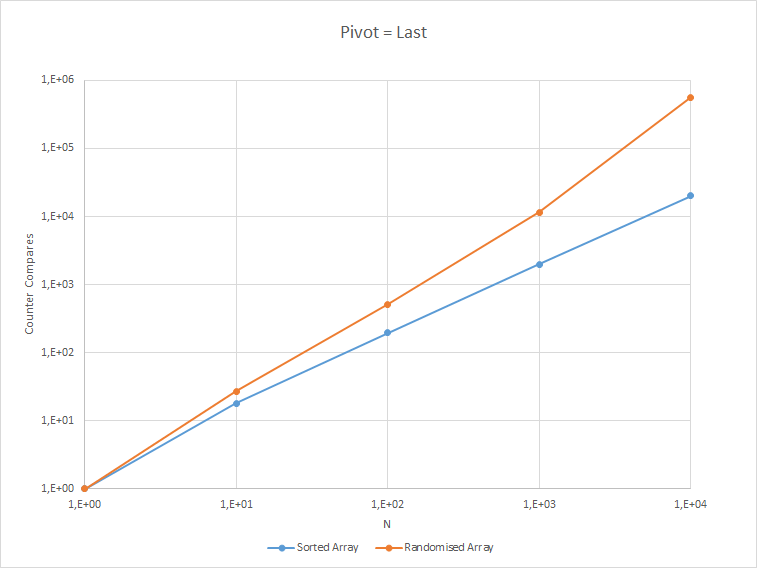
\includegraphics[width=0.49\textwidth]{pivotLast-counterCompares.png}} 
    \subfigure[Tauschen von Elementen]{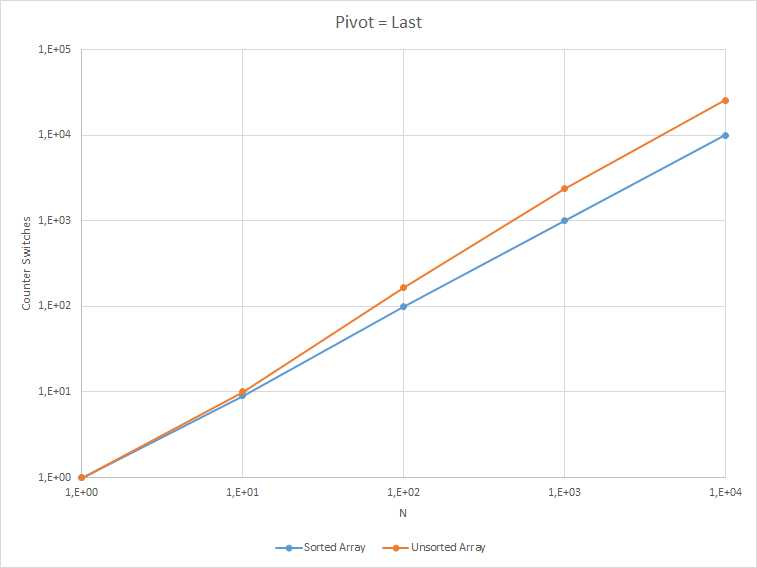
\includegraphics[width=0.49\textwidth]{pivotLast-counterSwitches.png}} 
\caption{Quicksort mit dem letzten Pivotelement} 
\end{figure} 

\newpage
\section{Median als Pivotelement}
Die zweite implementierte Methode zur Pivotwahl ist mit dem Median gelöst worden. Drei Elemente wurden dabei eingelesen, das erste, letzte, und welches sich auf mittlerer Position befindet. Diese werden nach dem zu sortierenden Attribut verglichen und der Median wird als Pivotelement gewählt. Dieses Vorgehen macht gleichmäßigere Aufteilung wahrscheinlicher, ohne die Aufwand zu erhöhen. Denn drei Elemente zu vergleichen ist ein konstanter Aufwand und hängt nicht von der Problemgröße ab.

\subsection{Tabellarische Darstellung}

\begin{table}[ht]
\centering
\caption{Quicksort mit dem Median-Pivotelement}
\begin{tabular}{r|c|c|c|c}
\multicolumn{1}{l|}{} & \multicolumn{2}{c|}{\textbf{Vergleiche}} & \multicolumn{2}{c|}{\textbf{Tausch}} \\ \hline
\rowcolor[HTML]{EFEFEF} 
\multicolumn{1}{l|}{\cellcolor[HTML]{EFEFEF}Größe} & Sortierte Liste & Zufällige Liste & Sortierte Liste & Zufällige Liste \\ \hline
1 & 0 & 0 & 0 & 0 \\ \hline
10 & 21 & 25 & 6 & 8 \\ \hline
100 & 360 & 556 & 63 & 146 \\ \hline
1000 & 5048 & 10796 & 511 & 2306 \\ \hline
10000 & 69017 & 561026 & 5904 & 25247
\end{tabular}
\end{table}
Dieses Untersuchungsergebnis, mit dem Median als Pivotelement bestätigt das Ergebnis aus der Untersuchung aus dem Punkt 2 (Seite 2). Die sortierte Liste stellt sich ebenfalls wieder als, der best-case, sowohl bei den Vergleichen, als auch bei den Tauschoperationen. 

\subsection{Grafik}
\begin{figure}[h] 
    \subfigure[Vergleiche zwischen Elementen]{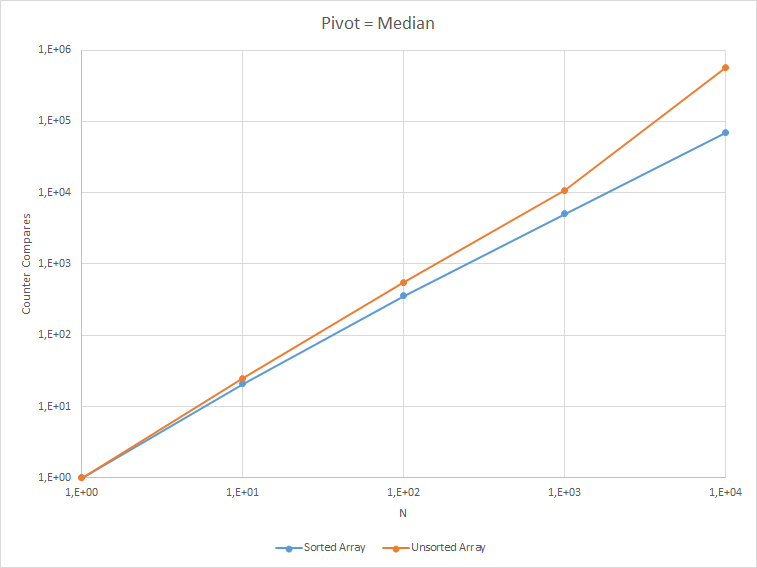
\includegraphics[width=0.49\textwidth]{pivotMedian-counterCompares.png}} 
    \subfigure[Tauschen von Elementen]{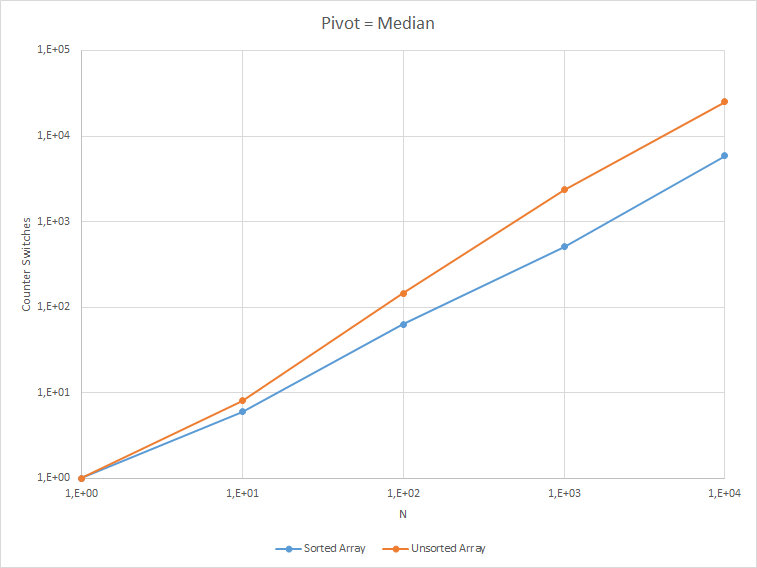
\includegraphics[width=0.49\textwidth]{pivotMedian-counterSwitches.png}} 
\caption{Quicksort mit dem Median-Pivotelement} 
\end{figure} 





\end{document}